\chapter{Results}

In this chapter, we evaluate the performance of the proposed autonomous highway driving system via computer simulations. It also briefly explains and discusses some characteristics of the results, whereas a more general discussion follows in the next Chapter. As described in Chapter 4, two agents with different action spaces were investigated. Agent 1 only decided when to change lanes, whereas Agent 2 decided both the speed and when to change lanes.

% Furthermore, two different neural network architectures were used.

%%%%%%%%%%%%%%%%%%%%%%%%%%%%%%%%%%%%%%%%%%%%%%%%%%%%%%%%%%%%%%%%%
\section{Simulation Setup}

In simulations, we used the open source software OpenAI-Gym and ROS / Gazebo which models highway environment in real time. We generated the environment in order to train the DQN by simulating the behaviors of the cars on highway. In the simulations, we assume that the positions and velocities of the ego vehicle's neighboring vehicles is detected and stored by the ego vehicle. In each episode, the initial position of ego vehicle is set to (0, -6) in the middle lane. The initial velocities of the other vehicle are set based on their lane. With different velocities, the other vehicles have chances to create several different scenarios for the DQN model to learn.

\begin{itemize}
\item Scenario 1: No vehicle in the ego vehicle's detecting range.
\item Scenario 2: One vehicle is detected in the same lane of the ego vehicle.
\item Scenario 3: One vehicle is detected but in a different lane of the ego vehicle.
\item Scenario 4: Vehicles are detected in the left, right and the ego's lanes.
\end{itemize}

%%%%%%%%%%%%%%%%%%%%%%%%%%%%%%%%%%%%%%%%%%%%%%%%%%%%%%%%%%%%%%%%%
\section{Training for Longitudinal Motion only}

\begin{figure}[h]
\centering
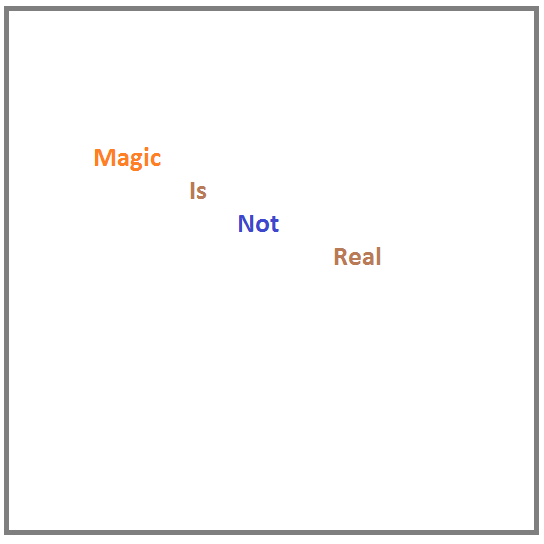
\includegraphics[width=1.0\textwidth]{figs/magic}
\caption{The architecture of Deep Neural Network.}
\label{fig:dnn}
\end{figure}

The neural network used for the DQN consists of the fully-connected layers with five hidden layers. RMSProp algorithm is used to minimize the loss with learning rate $\epsilon = 0.0005$. The number of position data samples used as a state is set to $n = 5$. We set the size of the replay memory to 10,000. We set the replay batch size to 32 and trauma batch size to 10. The summary of the DQN configurations used for our experiments is provided below:

\begin{itemize}
\item State buffer size: n = 5
\item Network architecture: fully-connected feed-forward network
\item Nonlinear function: leaky ReLU
\item Number of nodes for each layers : [17 (Input layer), 100, 70, 50, 70, 100, 27 (Output layer)]
\item RMSProp optimizer with learning rate 0.0005 [14]
\item Replay memory size: 10,000
\item Replay batch size: 32
\end{itemize}

\subsection{Case 1: The neighboring vehicles are at constant speeds.}

The parameters are set as below,

\begin{itemize}
\item Cruise speeds in Lane 0, 1and 2 are $vel_{lane0}, vel_{lane1}, vel_{lane2} = {12, 10, 8} m/s$ which means Lane 0, 1 and 2 are Fast Lane, Medium Lane and Slow Lane.
\item Safety distance is $dist_{safety} = 5 m$
\item $accel_{high}, accel_{low}, accel_{zero}, decel_{low}, decel_{high} = {2, 1, 0, -1, -2} m/s^2$
\end{itemize}

\begin{figure}[h]
\centering
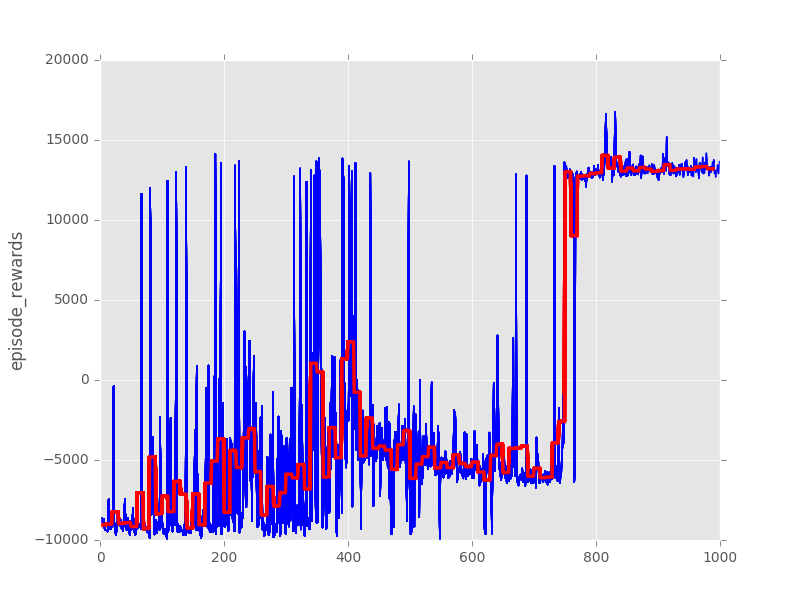
\includegraphics[width=1.0\textwidth]{figs/ch5/agent1-reward-history-epoch-1000-a}
\caption{The reward history of training for Adaptive Cruise Control in Case 1.}
\label{fig:res-1-a}
\end{figure}

Fig. \ref{fig:res-1-a} provides the plot of the total accumulated rewards i.e., value function achieved for each episode. We observe that the value function converges after 750 episodes and high total reward is steadily attained after convergence.

\subsection{Case 2: The neighboring vehicles are at erratic speeds.}

\begin{figure}[h]
\centering
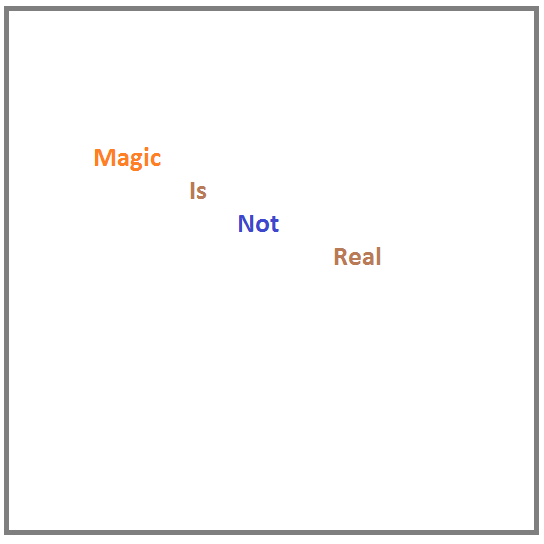
\includegraphics[width=0.5\textwidth]{figs/magic}
\caption{The speed variance of vehicle in each lane.}
\label{fig:erratic-curve}
\end{figure}

The parameters are set as below,

\begin{itemize}
\item The speed of the vehicle except for the ego vehicle in each lane would follow a sine curve, a period of zero value and a period of constant non-zero value as shown in Fig. \ref{fig:erratic-curve}.
\item Safety distance is  $dist_{safety} = 5 m$
\item $accel_{high}, accel_{low}, accel_{zero}, decel_{low}, decel{high} = {2, 1, 0, -1, -2} m/s^2$
\end{itemize}

\begin{figure}[h]
\centering
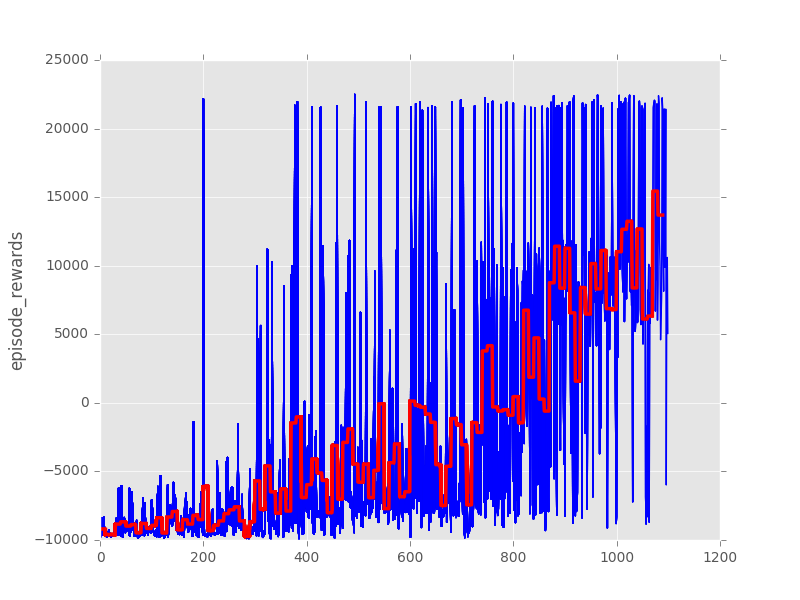
\includegraphics[width=1.0\textwidth]{figs/ch5/agent1-reward-history-epoch-1000-b}
\caption{The reward history of training for Adaptive Cruise Control in Case 2.}
\label{fig:res-1-b}
\end{figure}

Fig. \ref{fig:res-1-b} provides the plot of the total accumulated rewards i.e., value function achieved for each episode. We observe that the value function converges after 1,000 episodes and high total reward is steadily attained after convergence.

%%%%%%%%%%%%%%%%%%%%%%%%%%%%%%%%%%%%%%%%%%%%%%%%%%%%%%%%%%%%%%%%%
\section{Training for Lateral Motion only}

\begin{figure}[h]
\centering
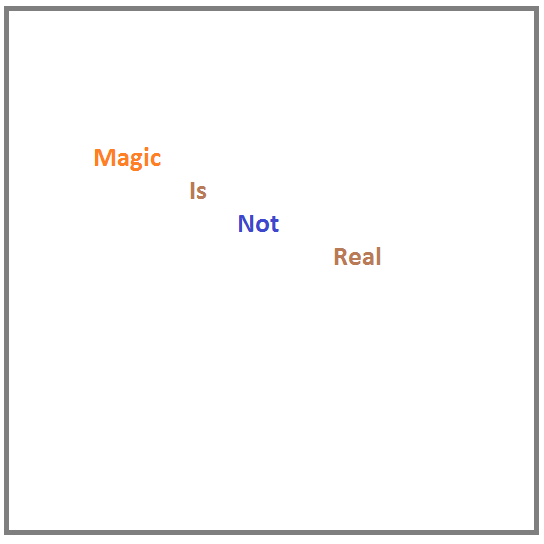
\includegraphics[width=1.0\textwidth]{figs/magic}
\caption{The architecture of Deep Neural Network.}
\label{fig:dnn}
\end{figure}

The neural network used for the DQN consists of the fully-connected layers with five hidden layers. RMSProp algorithm is used to minimize the loss with learning rate $\epsilon = 0.0005$. The number of position data samples used as a state is set to $n = 5$. We set the size of the replay memory to 10,000. We set the replay batch size to 32 and trauma batch size to 10. The summary of the DQN configurations used for our experiments is provided below:

\begin{itemize}
\item State buffer size: n = 5
\item Network architecture: fully-connected feed-forward network
\item Nonlinear function: leaky ReLU [13]
\item Number of nodes for each layers : [17 (Input layer), 100, 70, 50, 70, 100, 27 (Output layer)]
\item RMSProp optimizer with learning rate 0.0005 [14]
\item Replay memory size: 10,000
\item Replay batch size: 32
\end{itemize}

\subsection{Case 1: The neighboring vehicles are at constant speeds.}

The parameters are set as below,

\begin{itemize}
\item Cruise speeds in Lane 0, 1and 2 are $vel_{lane0}, vel_{lane1}, vel_{lane2} = {12, 10, 8} m/s$ which means Lane 0, 1 and 2 are Fast Lane, Medium Lane and Slow Lane.
\item Safety distance is $dist_{safety} = 5 m$
\item $accel_{high}, accel_{low}, accel_{zero}, decel_{low}, decel_{high} = {2, 1, 0, -1, -2} m/s^2$
\end{itemize}

\begin{figure}[h]
\centering
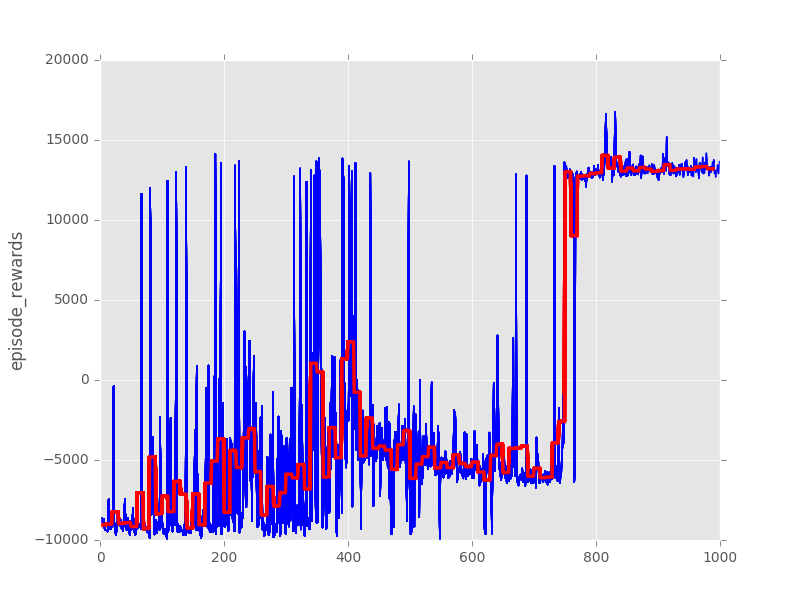
\includegraphics[width=1.0\textwidth]{figs/ch5/agent1-reward-history-epoch-1000-a}
\caption{The reward history of training for Adaptive Cruise Control in Case 1.}
\label{fig:res-1-a}
\end{figure}

Fig. \ref{fig:res-1-a} provides the plot of the total accumulated rewards i.e., value function achieved for each episode. We observe that the value function converges after 750 episodes and high total reward is steadily attained after convergence.

\subsection{Case 2: The neighboring vehicles are at erratic speeds.}

\begin{figure}[h]
\centering
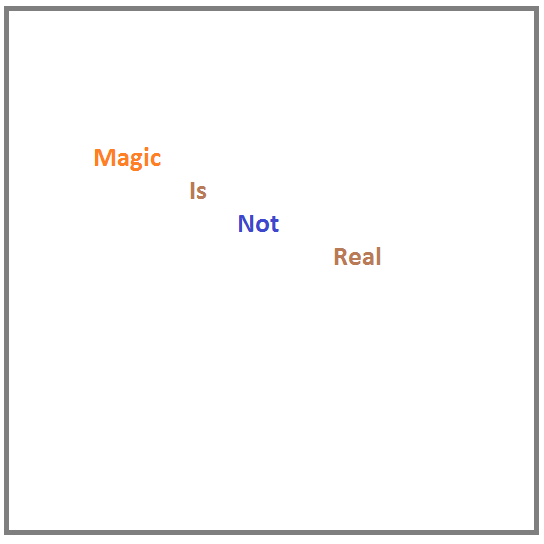
\includegraphics[width=0.5\textwidth]{figs/magic}
\caption{The speed variance of vehicle in each lane.}
\label{fig:erratic-curve}
\end{figure}

The parameters are set as below,

\begin{itemize}
\item The speed of the vehicle except for the ego vehicle in each lane would follow a sine curve, a period of zero value and a period of costant non-zero value as shown in Fig.  \ref{fig:erratic-curve}.
\item Safety distance is  $dist_{safety} = 5 m$
\item $accel_{high}, accel_{low}, accel_{zero}, decel_{low}, decel{high} = {2, 1, 0, -1, -2} m/s^2$
\end{itemize}

\begin{figure}[h]
\centering
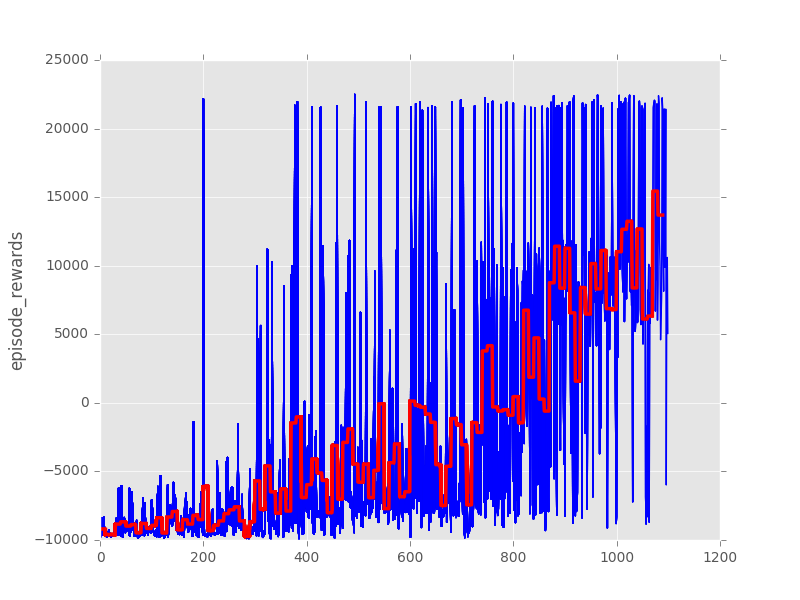
\includegraphics[width=1.0\textwidth]{figs/ch5/agent1-reward-history-epoch-1000-b}
\caption{The reward history of training for Adaptive Cruise Control in Case 2.}
\label{fig:res-1-b}
\end{figure}

Fig. \ref{fig:res-1-b} provides the plot of the total accumulated rewards i.e., value function achieved for each episode. We observe that the value function converges after 1,000 episodes and high total reward is steadily attained after convergence.

%%%%%%%%%%%%%%%%%%%%%%%%%%%%%%%%%%%%%%%%%%%%%%%%%%%%%%%%%%%%%%%%%
\section{Training for Combined Motion}

The neural network used for the DQN consists of the fully-connected layers with five hidden layers. RMSProp algorithm [14] is used to minimize the loss with learning rate ? = 0.0005. The number of position data samples used as a state is set to n = 5. We set the size of the replay memory to 10,000. We set the replay batch size to 32 and trauma batch size to 10. The summary of the DQN configurations used for our experiments is provided below:

\begin{itemize}
\item State buffer size: n = 5
\item Network architecture: fully-connected feed-forward network
\item Nonlinear function: leaky ReLU [13]
\item Number of nodes for each layers : [17 (Input layer), 100, 70, 50, 70, 100, 27 (Output layer)]
\item RMSProp optimizer with learning rate 0.0005 [14]
\item Replay memory size: 10,000
\item Replay batch size: 32
\end{itemize}

The parameters are set as below,

\begin{itemize}
\item Cruise speeds in Lane 0, 1and 2 are $vel_{lane0}, vel_{lane1}, vel_{lane2} = {12, 10, 8} m/s$ which means Lane 0, 1 and 2 are Fast Lane, Slow Lane.
\item Safety distance is $dist_{safety} = 5 m$
\item $accel_{high}, accel_{low}, accel_{zero}, decel_{low}, decel{high} = {2, 1, 0, -1, -2} m/s^2$
\end{itemize}

\begin{figure}[h]
\centering
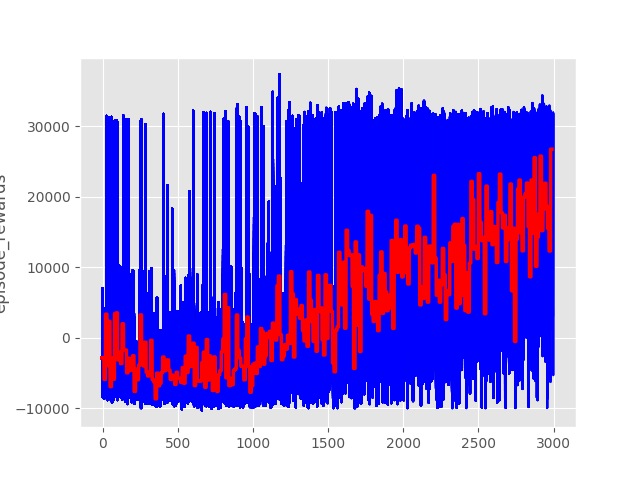
\includegraphics[width=1.0\textwidth]{figs/ch5/agent2-vehicle-reward-history-epoch-3000-std-track}
\caption{The reward history of training for full autonomous highway driving.}
\label{fig:res-2}
\end{figure}

Fig. \ref{fig:res-2} provides the plot of the total accumulated rewards i.e., value function achieved for each episode. We observe that the value function converges after 2,000 episodes and high total reward is steadily attained after convergence.

Both Agent1FCNN and Agent2FCNN failed to complete all the evaluation episodes without collisions, see Fig. 4 and Table VI. Naturally, Agent1FCNN solved a significantly higher fraction of the episodes and performed better than Agent2FCNN, since it only needed to decide when to change lanes, and not control the speed. In the beginning, it learned to always stay in its lane, and thereby solved all episodes without collisions, but reached a lower performance index than the reference model, see Fig. 5. With more training, it started to change lanes and performed reasonably well, but sometimes caused collisions. Agent2FCNN performed significantly worse and collided in 14\% of the episodes by the end of its training. A longer training run was carried out for Agent1FCNN and Agent2FCNN, but after 20 million iterations, the results were the same.

%\vfill
